\setcounter{section}{-1}



\section{Preliminaries(预备知识)}

\frame{
\frametitle{Derivative $\&$ Antiderivative}
\framesubtitle{导数和不定积分}
\begin{block}{Consider the function $f(x) = \cos(x)$, }
\begin{itemize}
\item its derivative $f′(x) = - \sin(x)$, 
\item and its antiderivative $F(x) = \sin(x) + C$. 
\end{itemize}
\end{block}
\begin{block}{These formulas were studied in calculus.}
\begin{itemize}
\item The former is used to determine the slope $m = f'(x_0)$ of the curve $y = f (x)$ at a point $(x_0, f(x_0))$;
\item The latter is used to compute the area under the curve for $a \le x \le b$.
\end{itemize}
\end{block}
}

\frame{
 \begin{itemize}
\item The slope at the point $(\pi \slash 2, 0)$ is $m = f'(\pi \slash 2) = −1$ and can be used to find the tangent line at this point :
\begin{equation*}
y_{tan} = m\left( x - \frac{\pi}{2}\right) + 0 
= f' \left(\frac{\pi}{2} \right)\left(x-\frac{\pi}{2} \right)
= -x + \frac{\pi}{2}
\end{equation*}
\item The area under the curve for $ 0 \le x \le \pi \slash 2$ is computed using an integral :
\begin{equation*}
area = \int_0^{\pi \slash 2} \cos (x) dx
= F \left( \pi \slash 2 \right) -F(0) = \sin\left( \frac{\pi}{2} \right) - 0 
= 1 
\end{equation*}
\end{itemize}
\begin{columns}
\begin{column}{0.5\textwidth}
\begin{figure}
\begin{center}
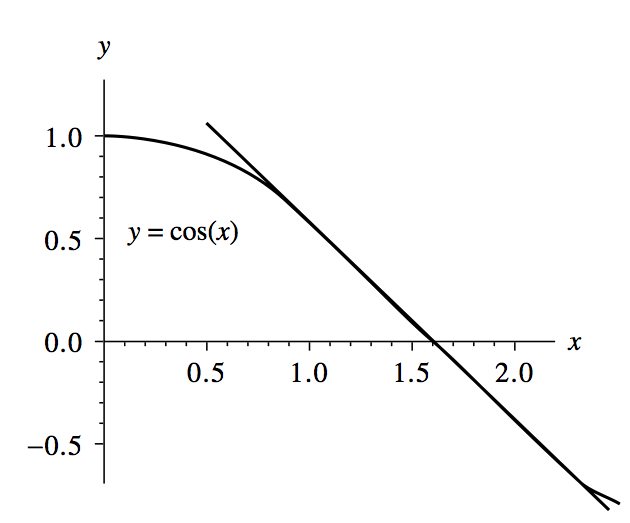
\includegraphics[width=40mm]{chap-0/fig_1-1.png}
{\tiny  \\ The tangent line to the curve $y = cos(x)$ at the point $(\pi \slash 2, 0)$.}	
\end{center}
\end{figure}
\end{column}
\begin{column}{0.5\textwidth}
\begin{figure}
\begin{center}
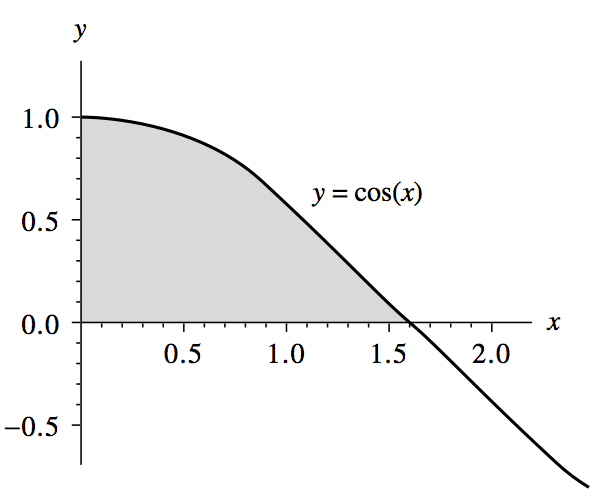
\includegraphics[width=40mm]{chap-0/fig_1-1_2.png}
{\tiny  \\ The area under the curve 
$y = \cos(x)$ 
over the interval
$[ 0, \pi \slash 2 ]$.}
\end{center}
\end{figure}
\end{column}
\end{columns}
}


\subsection{Review of Calculus}

\frame{
\begin{block}{}
\begin{itemize}
\item It is assumed that the reader is familiar with the notation and subject matter covered in the undergraduate calculus sequence. 
\vspace{0.5cm}
\item This should have included the topics :
\vspace{0.2cm}
\begin{itemize} 
\item limits (极限), 
\vspace{0.2cm}
\item continuity (连续), 
\vspace{0.2cm}
\item differentiation (微分), 
\vspace{0.2cm}
\item integration (积分), 
\vspace{0.2cm}
\item sequences (序列), 
\vspace{0.2cm}
\item series (级数).  
\end{itemize}
\end{itemize}
\end{block}
}

\frame{
\frametitle{Limits and Continuity}
\framesubtitle{极限和连续}
\begin{figure}
\begin{center}
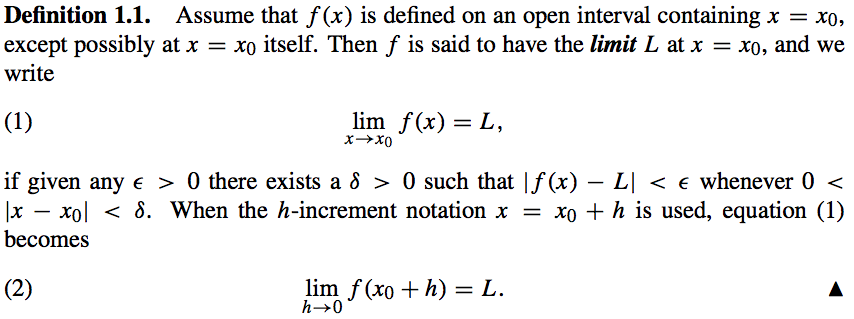
\includegraphics[width=115mm]{chap-0/def_1-1.png}
\end{center}
\end{figure}
\begin{block}{极限的定义}
例如,该定义主要是应用在本课程的非线性方程的迭代算法。
\end{block}
}

\frame{
\begin{figure}
\begin{center}
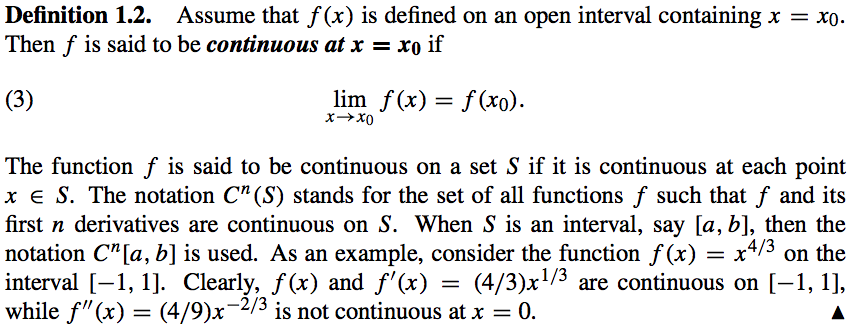
\includegraphics[width=115mm]{chap-0/def_1-2.png}
\end{center}
\end{figure}
\begin{block}{连续的定义}
注意与本课程之中所应用的离散数据的相似性和差别。
\end{block}
}

\frame{
\begin{figure}
\begin{center}
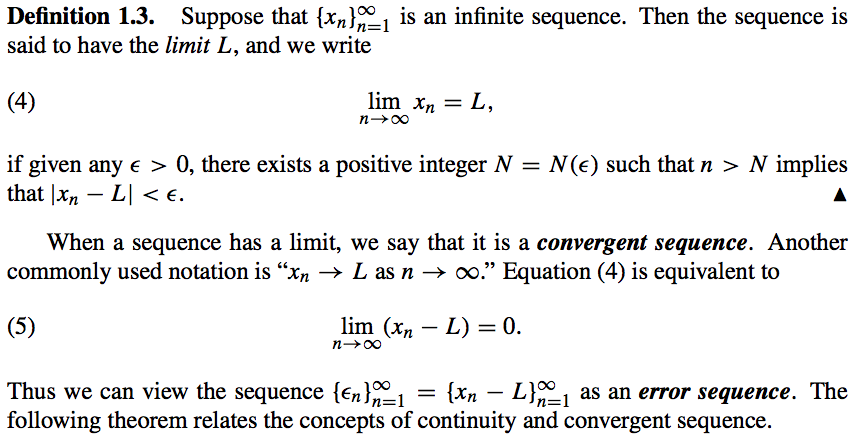
\includegraphics[width=115mm]{chap-0/def_1-3.png}
\end{center}
\end{figure}
\begin{block}{序列的收敛性定义}
由于计算机的数据存储是离散的,该定义在本课程之中具有实际意义。
\end{block}
}

\frame{
\begin{figure}
\begin{center}
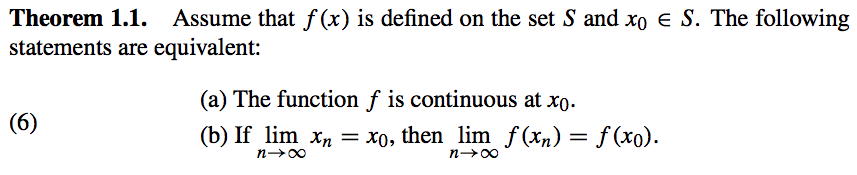
\includegraphics[width=115mm]{chap-0/the_1-1.png}
\end{center}
\end{figure}
\begin{block}{}
%由于计算机的数据存储是离散的,该定义在本课程之中具有实际意义。
\end{block}

\begin{figure}
\begin{center}
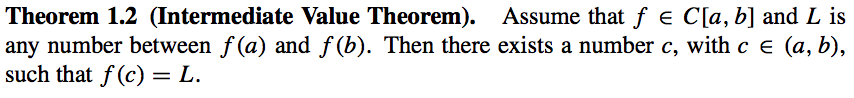
\includegraphics[width=115mm]{chap-0/the_1-2.png}
\end{center}
\end{figure}
\begin{block}{}
\end{block}
}

\frame{
\begin{figure}
\begin{center}
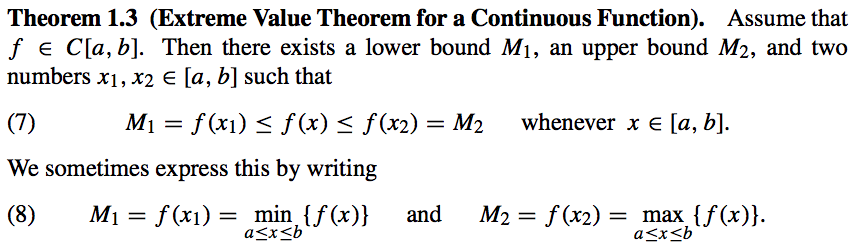
\includegraphics[width=115mm]{chap-0/the_1-3.png}
\end{center}
\end{figure}
\begin{block}{连续函数的极值定理}
\end{block}
}

\frame{
\frametitle{Differentiable Functions}
\framesubtitle{可微函数}
\begin{figure}
\begin{center}
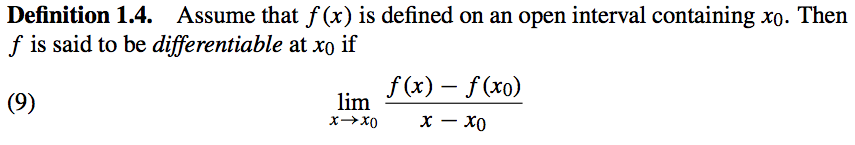
\includegraphics[width=115mm]{chap-0/def_1-4.png}
\end{center}
\end{figure}
\begin{figure}
\begin{center}
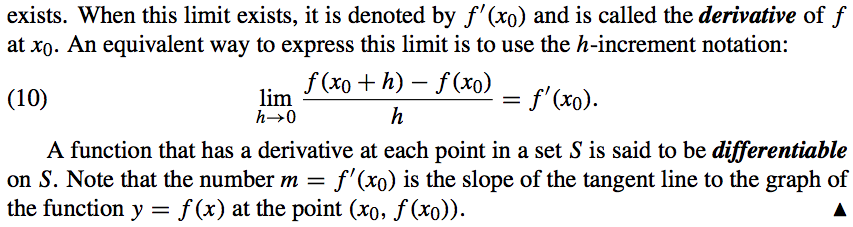
\includegraphics[width=115mm]{chap-0/def_1-4_2.png}
\end{center}
\end{figure}
\begin{block}{函数可导的定义}
可以利用该定义计算函数曲线的微分曲线。
\end{block}
}

\frame{
\begin{figure}
\begin{center}
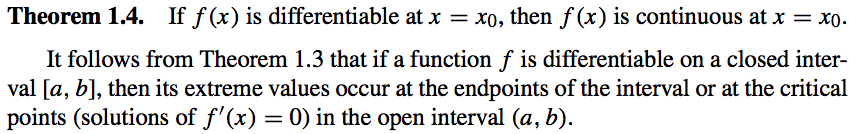
\includegraphics[width=115mm]{chap-0/the_1-4.png}
\end{center}
\end{figure}
\begin{block}{可导和连续的关系}
\begin{itemize}
\item 如果函数在指定点可导的话一定连续,
\item 但如果函数在指定点连续的话不一定可导
\end{itemize}
\end{block}
}

\frame{
\begin{figure}
\begin{center}
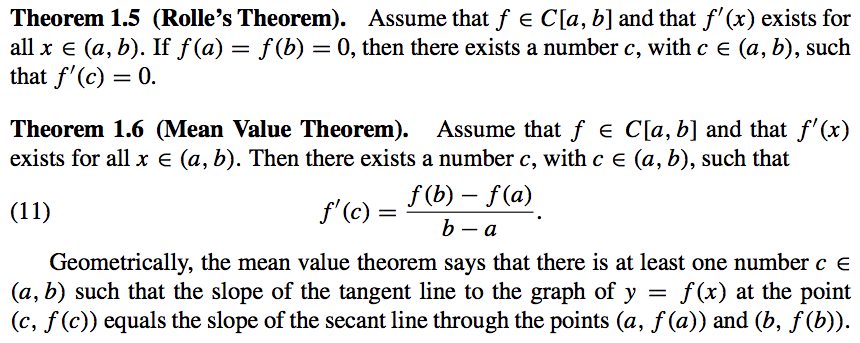
\includegraphics[width=115mm]{chap-0/the_1-5.png}
\end{center}
\end{figure}
\begin{block}{Rolle's theorem(罗尔定理) 和均值定理}
该定理可用在数值积分的推导之中
\end{block}
}

\frame{
\begin{figure}
\begin{center}
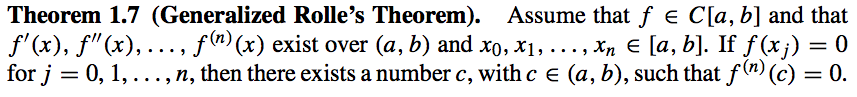
\includegraphics[width=115mm]{chap-0/the_1-7.png}
\end{center}
\end{figure}
\begin{block}{Generalized Rolle's theorem(广义罗尔定理) }
该定理是微分中值定理中最基本、最重要的,其证明具有广泛的代表性。
\end{block}
}

\frame{
\frametitle{Integrals}
\framesubtitle{积分}
\begin{figure}
\begin{center}
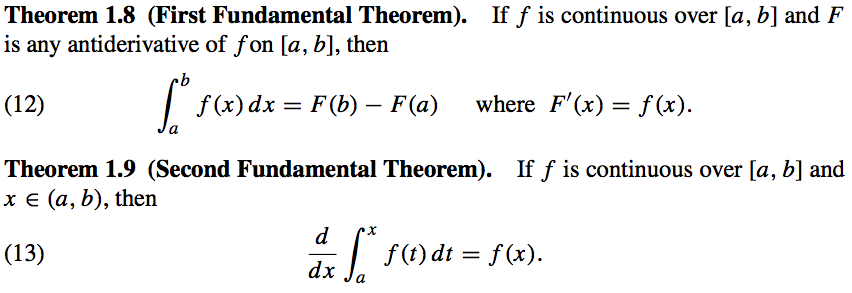
\includegraphics[width=115mm]{chap-0/the_1-8.png}
\end{center}
\end{figure}
\begin{block}{积分第一定理和第二定理}
该定理被应用在在本课程的数值积分。
\end{block}
}

\frame{
\begin{figure}
\begin{center}
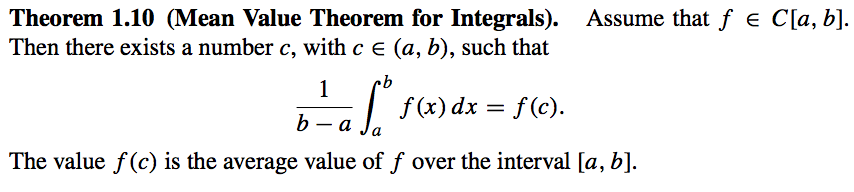
\includegraphics[width=115mm]{chap-0/the_1-10.png}
\end{center}
\end{figure}
\begin{block}{积分中值定理}
\end{block}
\begin{figure}
\begin{center}
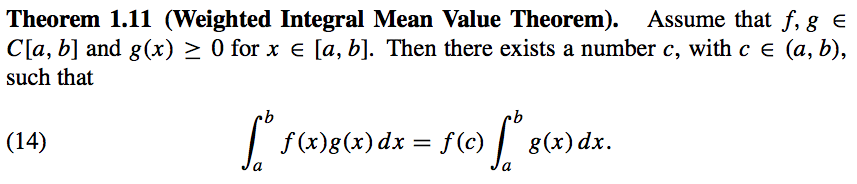
\includegraphics[width=115mm]{chap-0/the_1-11.png}
\end{center}
\end{figure}
\begin{block}{积分加权中值定理}
\end{block}
}

\frame{
\frametitle{Series}
\framesubtitle{级数}
\begin{figure}
\begin{center}
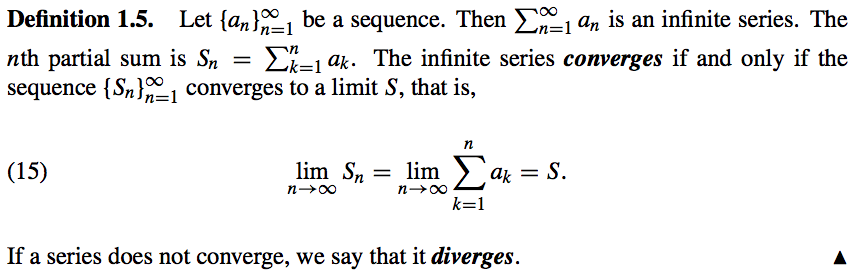
\includegraphics[width=115mm]{chap-0/def_1-5.png}
\end{center}
\end{figure}
\begin{block}{}
收敛和发散的定义
\end{block}
}

\frame{
\frametitle{Taylor's Theorem}
\framesubtitle{泰勒定理}
\begin{figure}
\begin{center}
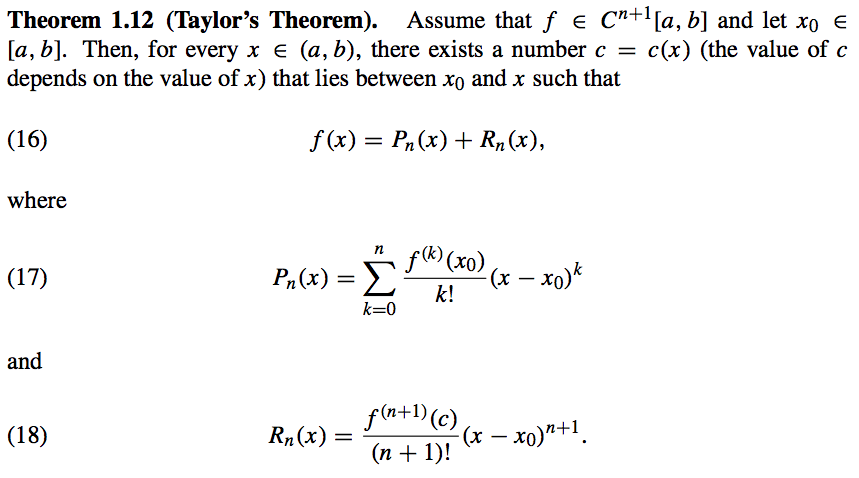
\includegraphics[width=115mm]{chap-0/the_1-12.png}
\end{center}
\end{figure}
}

\frame{
\frametitle{Corollary of the Taylor's Theorem}
\framesubtitle{泰勒定理的推理}
\begin{figure}
\begin{center}
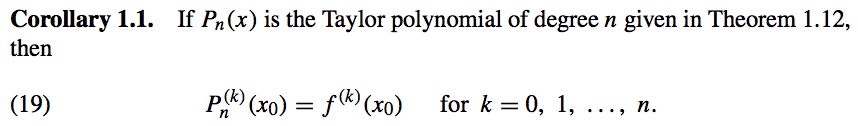
\includegraphics[width=115mm]{chap-0/coro_1-1.png}
\end{center}
\end{figure}
}

\frame{
\frametitle{Evaluation of a Polynomial}
\framesubtitle{多项式估值}
\begin{figure}
\begin{center}
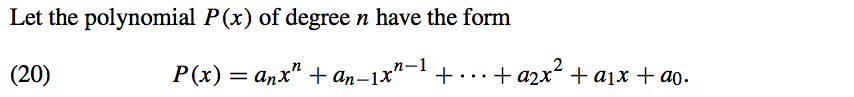
\includegraphics[width=115mm]{chap-0/p_19.png}
\end{center}
\end{figure}
\begin{figure}
\begin{center}
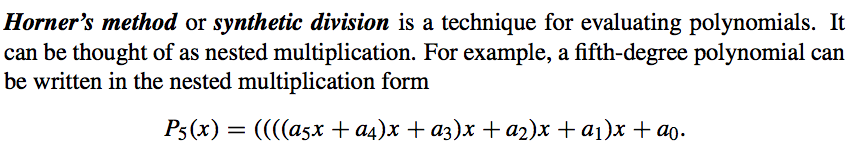
\includegraphics[width=115mm]{chap-0/p_19_2.png}
\end{center}
\end{figure}
}

\frame{
\begin{figure}
\begin{center}
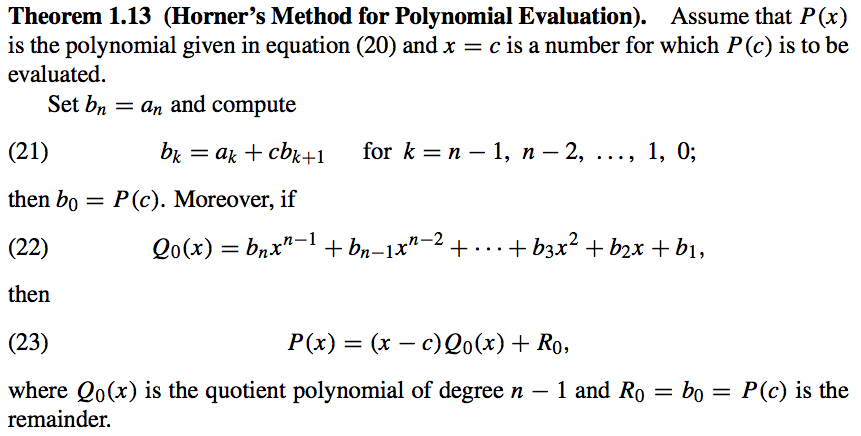
\includegraphics[width=115mm]{chap-0/the_1-13.png}
\end{center}
\end{figure}
}

\frame{
\begin{figure}
\begin{center}
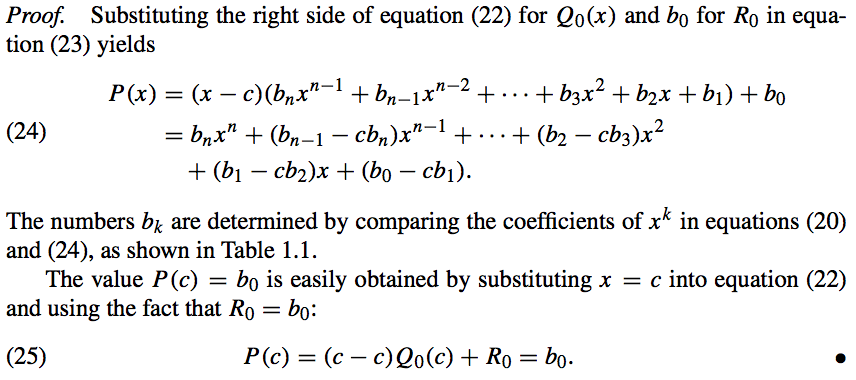
\includegraphics[width=115mm]{chap-0/the_1-13_2.png}
\end{center}
\end{figure}
}



\subsection{Binary Numbers(二进制数)}

\frame{
\begin{block}{}
\begin{itemize}
\item Human beings do arithmetic using the decimal (base 10) number system. 
\item Most computers do arithmetic using the binary (base 2) number system. 
\end{itemize}
\end{block}
\begin{itemize}
\item It may seem otherwise, 
since communication with the computer (input/output) is in base 10 numbers. 
\item This transparency does not mean that the computer uses base 10. 
\item In fact, it converts inputs to base 2 (or perhaps base 16), then performs base 2 arithmetic, and finally, translates the answer into base 10 before it displays a result. 
\end{itemize}
}

\frame{
\frametitle{Base 10 Number}
\begin{figure}
\begin{center}
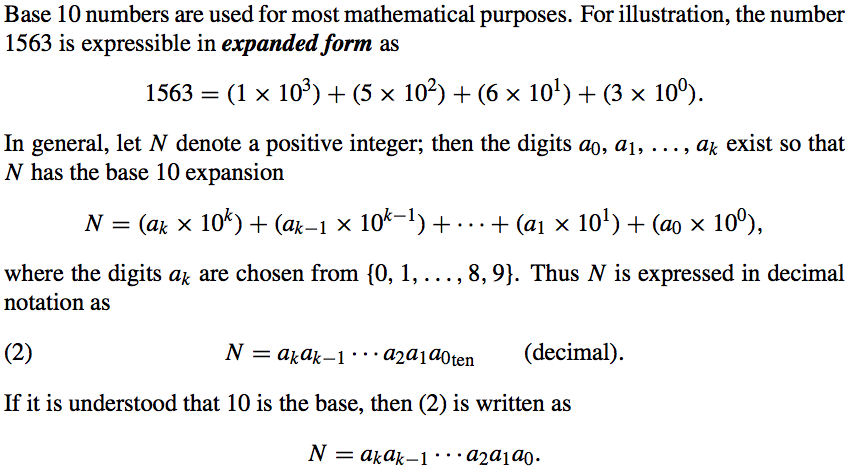
\includegraphics[width=115mm]{chap-0/p_24.png}
\end{center}
\end{figure}
}

\frame{
\frametitle{Base 2 Number}
\begin{figure}
\begin{center}
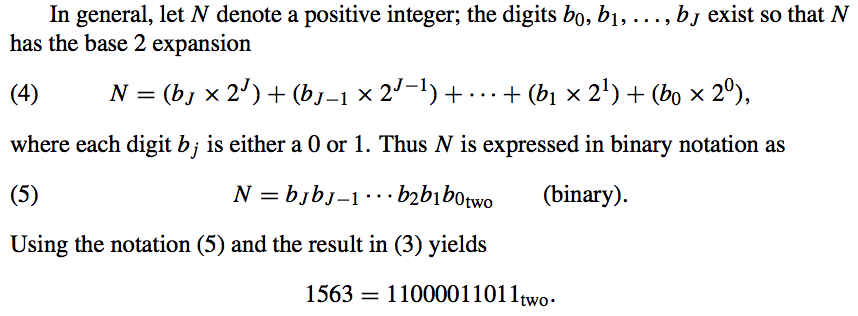
\includegraphics[width=115mm]{chap-0/p_24_2.png}
\end{center}
\end{figure}
}

\frame{
\frametitle{Sequences and Series}
\begin{figure}
\begin{center}
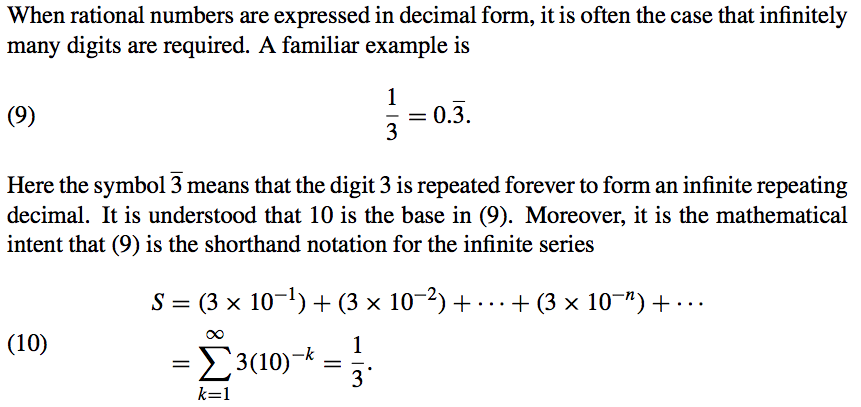
\includegraphics[width=115mm]{chap-0/p_26.png}
\end{center}
\end{figure}
}

\frame{
\begin{figure}
\begin{center}
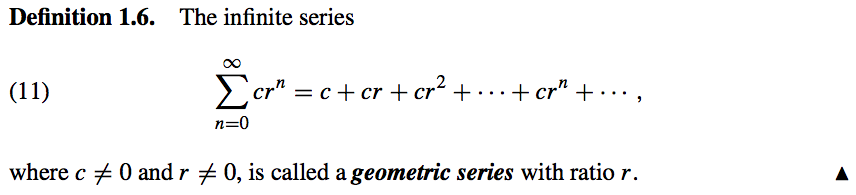
\includegraphics[width=115mm]{chap-0/def_1-6.png}
\end{center}
\end{figure}
\begin{figure}
\begin{center}
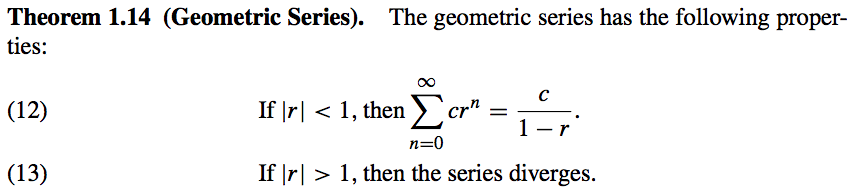
\includegraphics[width=115mm]{chap-0/the_1-14.png}
\end{center}
\end{figure}
}

%\frame{
%\frametitle{Computer Accuracy}
%\framesubtitle{计算机精度}
%\begin{itemize}
%\itemTo store numbers accurately, computers must have floating-point binary numbers %with at least 24 binary bits used for the mantissa; 
%\item this translates to about seven decimal places. 
%\item If a 32-bit mantissa is used, numbers with nine decimal places can be stored. 
%\end{itemize}
%}





\subsection{Error Analysis(误差分析)}

\frame{
\begin{block}{Error Analysis}
\begin{itemize}
\item In the practice of numerical analysis it is important to be aware that computed solutions are not exact mathematical solutions. 
\vspace{0.3cm}
\item The precision of a numerical solution can be diminished in several subtle ways. 
\vspace{0.3cm}
\item Understanding these difficulties can often guide the practitioner in the proper implementation and/or development of numerical algorithms.
\end{itemize}
\end{block}
}

\frame{
\begin{center}
{\Huge Computers are only as good as the person running them.}
\end{center}
}

\frame{
\frametitle{Numerical Errors}
\begin{itemize}
\item Precision Limits(精度限制)
\item Stability
\begin{itemize}
\item Convergence(收敛)
\item Divergence (发散)
\end{itemize}
\item Round-off Errors
\item Truncation Errors $-$ Code dependent
\item Machine Precision
\end{itemize}
\begin{block}{误差来源}
\begin{itemize}
\item 模型误差: 在建立数学模型过程中,不可能将所有因素均考虑,必然要进行必要的简化,这就带来了与实际问题的误差。
\item 观测误差: 测量已知参数时,数据带来的误差。工程问题的参数包含有不可避免的测量误差。
\item 截断误差:数值方法的精确解与待求解模型的理论分析解之间的差异
\item 舍入误差:对超过某有限位数的数据进行舍入所产生的误差
\end{itemize}
\end{block}
}

\frame{
\frametitle{Absolute $\&$ Relative errors}
\framesubtitle{绝对误差和相对误差}
\begin{figure}
\begin{center}
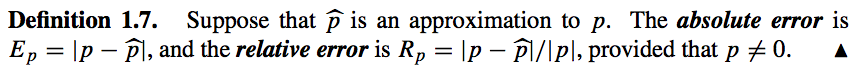
\includegraphics[width=115mm]{chap-0/def_1-7.png}
\end{center}
\end{figure}
\begin{block}{Example}
Let $x = 3.141592$ and $ \hat{x} = 3.14 $
\begin{itemize}
\item $ E_x = |x - \hat{x}| = |3.141592 - 3.14| = 0.001592 $
\vspace{0.3cm}
\item $ R_x = \frac{|x - \hat{x}|}{|x|}  = \frac{0.001592}{3.141592} = 0.00507 $
\end{itemize}
\end{block}
}

\frame{
\frametitle{Truncation Error}
\framesubtitle{截断误差}
\begin{figure}
\begin{center}
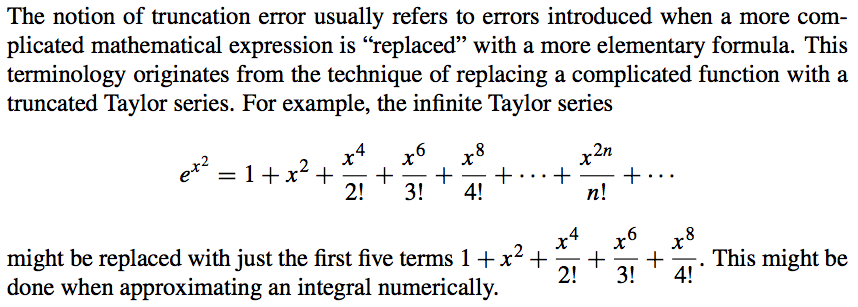
\includegraphics[width=115mm]{chap-0/p_36.png}
\end{center}
\end{figure}

}

\frame{
\frametitle{Round-off Error}
\framesubtitle{舍入误差}
\begin{block}{}
\begin{itemize}
\item A computer’s representation of real numbers is limited to the fixed precision of the mantissa. 
\item True values are sometimes not stored exactly by a computer’s represen- tation. This is called round-off error.
\end{itemize}
\end{block}
\begin{block}{}
\begin{itemize}
\item In the preceding section the real number $1/10 = 0.0\bar{0011}_{two} $ was truncated when it was stored in a computer. 
\item The actual number that is stored in the computer may undergo chopping or rounding of the last digit. 
\item Therefore, since the computer hardware works with only a limited number of digits in machine numbers, rounding errors are introduced and propagated in successive computations.
\end{itemize}
\end{block}
}

\frame{
\frametitle{误差界 $\&$ 误差限}
\begin{block}{}
设$x$为准确值,
$x^{\ast}$为$x$的一个近似值,
若
\begin{equation*}
| e | = | x - x^{\ast} | \le  \epsilon
\end{equation*}
则$\epsilon$为$x^{\ast}$的绝对误差界,简称误差界。\\
若
\begin{equation*}
|e_r| = \frac{| x - x^{\ast} |}{| x^{\ast} |}  \le  \epsilon_r
\end{equation*}
则$\epsilon_r$为$x^{\ast}$的相对误差界。\\
\end{block}
\begin{block}{}
引入$\epsilon$误差界的定义,可以把无法明明白白写出来得准确值$x$表示为:
\begin{equation*}
 x^{\ast}  - \epsilon  \le  x  \le  x^{\ast}  + \epsilon
\hspace{1cm} 或 \hspace{1cm} 
x  =   x^{\ast}  \pm \epsilon
\end{equation*}
\end{block}
}

\frame{
\frametitle{Significant digits}
\framesubtitle{有效数字}
\begin{figure}
\begin{center}
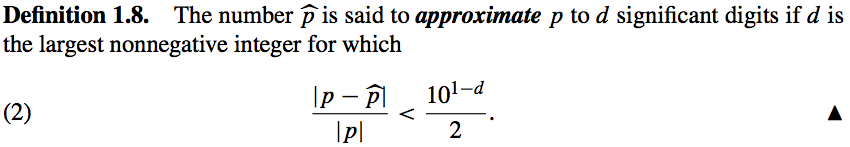
\includegraphics[width=115mm]{chap-0/def_1-8.png}
\end{center}
\end{figure}
\begin{block}{Example}
If $x = 3.141592$ and $\hat{x} = 3.14$,  \\
then $\frac{|x - \hat{x}|}{|x|} = 0.000507 < \frac{10^{-2}}{2}$. \\
Therefore, $\hat{x}$ approximates $x$ to two significant digits.
\end{block}
}



\frame{
\frametitle{Loss of Significance}
\framesubtitle{精度损失}
Consider the two numbers $p = 3.1415926536$ and $q = 3.1415957341$, which are nearly equal and both carry 11 decimal digits of precision. 
\begin{itemize}
\item Suppose that their difference is formed: $p - q = −0.0000030805$. 
\item Since the first six digits of $p$ and $q$ are the same, their difference $p - q$ contains only five decimal digits of precision. 
\item This phenomenon is called loss of {\large significance} or {\large subtractive cancellation}. 
\item This reduction in the precision of the final computed answer can creep in when it is not suspected.
\end{itemize}
\begin{block}{}
For polynomial evaluation, the rearrangement of terms into nested multiplication form will sometimes produce a better result.
\end{block}
}

\frame{
\frametitle{$O(h^n)$ Order of Approximation}
\framesubtitle{$O(h^n)$阶逼近}
\begin{figure}
\begin{center}
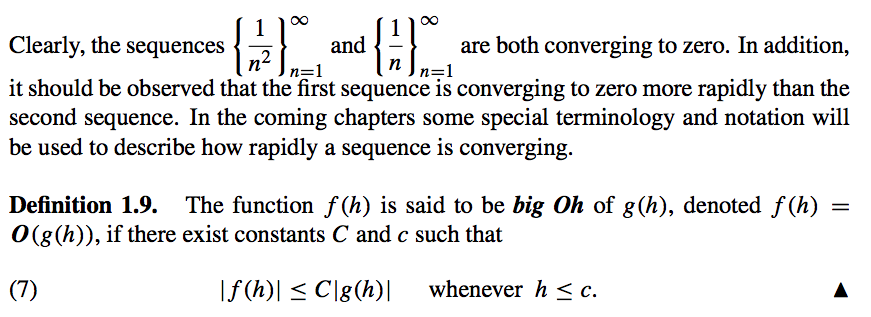
\includegraphics[width=115mm]{chap-0/def_1-9.png}
\end{center}
\end{figure}
}

\frame{
\frametitle{$O(h^n)$ Order of Approximation}
\framesubtitle{$O(h^n)$阶逼近}
\begin{figure}
\begin{center}
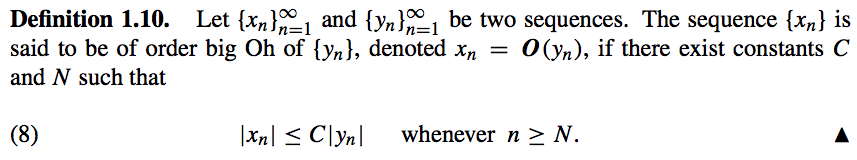
\includegraphics[width=115mm]{chap-0/def_1-10.png}
\end{center}
\end{figure}
\begin{figure}
\begin{center}
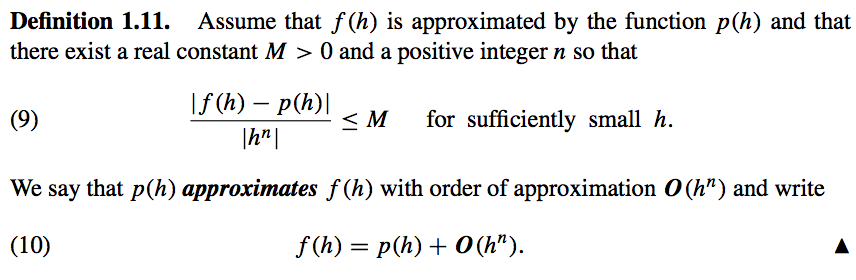
\includegraphics[width=115mm]{chap-0/def_1-11.png}
\end{center}
\end{figure}
}

\frame{
\begin{figure}
\begin{center}
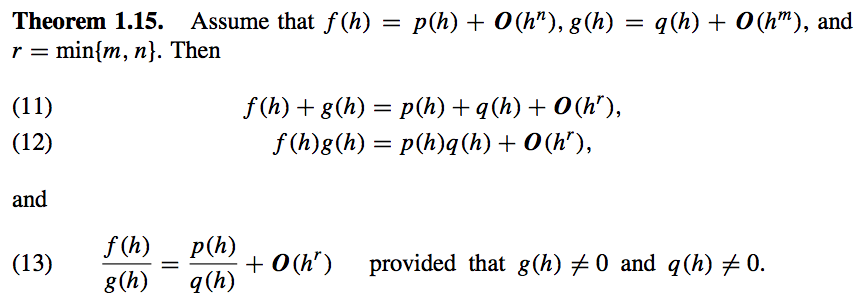
\includegraphics[width=115mm]{chap-0/the_1-15.png}
\end{center}
\end{figure}
\begin{figure}
\begin{center}
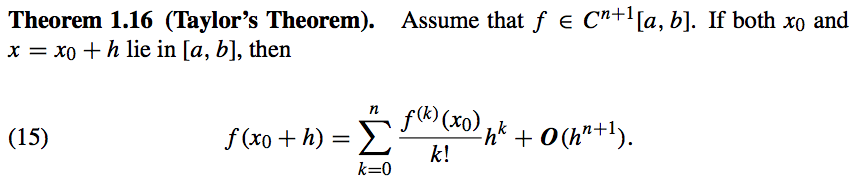
\includegraphics[width=115mm]{chap-0/the_1-16.png}
\end{center}
\end{figure}
}


\frame{
\frametitle{Order of Convergence of a Sequence}
\begin{itemize}
\item Numerical approximations are often arrived at by computing a sequence of approximations that get closer and closer to the answer desired. 
\item The definition of big $Oh$ for sequences was given in Definition 1.10, and the definition of order of convergence for a sequence is analogous to that given for functions in Definition 1.11.
\end{itemize}
\begin{figure}
\begin{center}
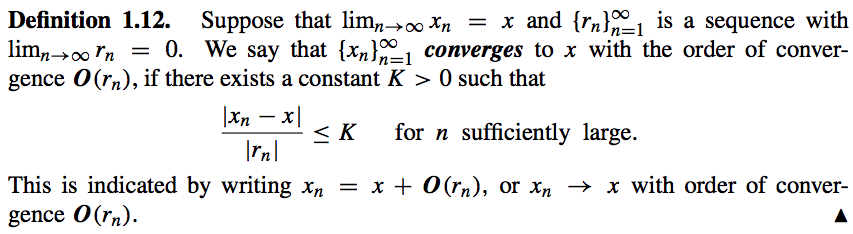
\includegraphics[width=115mm]{chap-0/def_1-12.png}
\end{center}
\end{figure}
}



\frame{
\frametitle{Uncertainty in Data}
\begin{itemize}
\item Data from real-world problems contain uncertainty or error. 
\item This type of error is referred to as noise. 
\item It will affect the accuracy of any numerical computation that is based on the data. 
\item An improvement of precision is not accomplished by performing succes- sive computations using noisy data. 
\item Hence, if you start with data with d significant digits of accuracy, then the result of a computation should be reported in d significant digits of accuracy. 
\end{itemize}
}

\frame{
For example,
\begin{itemize}
\item suppose that the data $p_1 = 4.152$ and $p_2 = 0.07931$ both have four significant digits of accuracy. 
\item Then it is tempting to report all the digits that appear on your calculator (i.e., $p_1 + p_2 = 4.23131$). 
\item This is an oversight, because you should not report conclusions from noisy data that have more significant digits than the original data. 
\item The proper answer in this situation is $p_1 + p_2 = 4.231$.
\end{itemize}
}


\subsection{Matlab $-$ Matrix Laboratory}

\frame{
\frametitle{Matlab的起源}
\begin{itemize}
\item 20世纪七十年代,时任美国新墨西哥大学计算机科学系主任的Cleve Moler出于减轻学生编程负担的动机, 为学生设计了一组调用LINPACK和EISPACK矩阵软件工具包库程序的的“通俗易用”的接口,此即用FORTRAN编写的萌芽状态的MATLAB。
\item 1984年由Little、Moler、Steve Bangert合作成立MathWorks公司,并把MATLAB正式推向市场。从这时起,MATLAB的内核采用C语言编写,而且除原有的数值计算能力外,还新增了数据图视功能。
\item 取名MATLAB即Matrix Laboratory 矩阵实验室的意 思。
\end{itemize}
}

\frame{
\frametitle{Matlab的特点}
\begin{itemize}
\item MATLAB是一种直译式的高级语言,比其它程序设计语言容易。
\item MATLAB语言是功能强大的计算机高级语言, 它以超群的风格与性能风靡全世界, 成功地应用于各工程学科的研究领域。 MATLAB在美国已经作为大学工科学生必修的计算机语言之一(C, FORTRAN, ASSEMBLER, MATLAB)。
\item MATLAB提供了丰富的矩阵运算处理功能,是基于矩阵运算的处理工具。
\end{itemize}
}

\frame{
\frametitle{主要应用领域}
\begin{itemize}
\item 工业研究与开发 ␣ 
\item 数学教学,特别是线性代数 
\item 数值分析、 信号处理和科学计算方面的教学与研究
\item 电子学、控制理论和物理学等工程和科学学科方面的教学与研究
\item 经济学、化学和生物学等计算问题的所有其他领域中的教学与研究
\end{itemize}
}


\frame{
%The Matlab program can be run using command line,  batch commands, and programs.
\begin{block}{Variable Types}
\begin{itemize}
\item Integers
\item Real Values (float and double)
\item Complex Numbers ($a + ib$)
\begin{itemize}
\item a $-$ real value
\item b $-$ imaginary value ($i$ is the square root of $-1$)   
\end{itemize}
\end{itemize}
\end{block}
\begin{block}{Data Types}
\begin{itemize}
\item Numerical
\begin{itemize}
\item Scalars
\item Vectors
\item Matrices
\end{itemize}
\item Logic Types
\item Alpha/Numerical Types
\end{itemize}
\end{block}
}

\frame{
\begin{itemize}
\item A scalar value is the simple number, $a$, $2$, $3.14157$ $\ldots$, 
\item A vector is a union of a
\end{itemize}
\begin{equation*}  
\bar{x} = \left\{ x_1, x_2, \ldots, x_n \right\} 
\end{equation*}
\begin{itemize}					
\item Transpose vector
\end{itemize}
\begin{equation*}
\bar{x}^T = \left\{
\begin{array}{c}
 x_1 \\
 x_2 \\
 \vdots \\
 x_n
\end{array} 
\right\}
\end{equation*}
}

\frame{
\begin{block}{Matrix is a combination of vectors and scalars.  Scalar and vectors are subsets of matrices.}
\begin{equation*}
A = \left[
\begin{array}{c c c c}
a_{11}  & a_{12}  & \cdots & a_{1n} \\
a_{21}  & a_{22}  & \cdots & a_{2n} \\
\vdots & \vdots & \ddots & \vdots \\ 
a_{n1}  & a_{n2}  & \cdots & a_{nn} \\
\end{array}
\right]
\end{equation*}
Matlab uses matrix to do mathematical methods.
\end{block}
}

\frame{
\begin{block}{Set of computer functions}
\begin{itemize}
\item Circular functions 
\begin{itemize}
\item $sin(x)$, $cos(x)$, $tan(x)$
\item $asin(x)$, $acos(x)$, $atan(x)$
\end{itemize}
\item Hyperbolic functions   
\begin{itemize}
\item $sinh(x)$, $cosh(x)$, $tanh(x)$
\end{itemize}
\item Logarithmic functions 
\begin{itemize}
\item $ln(x)$, $log(x)$ 
\item $exp(x)$
\end{itemize}
\item Logic functions           
\begin{itemize}
\item $abs(x)$
\item $real(x)$, $imag(x)$
\end{itemize}
\end{itemize}
\end{block}
}

\frame{
\begin{block}{Simple commands}
\begin{itemize}
\item clc     $-$ clears window
\item clg     $-$ clear graphic window
\item clear  $-$ clears the workspace
\item who	 $-$ variable list
\item whos $-$ variable list with size
\item help	 $-$ when doubt use it!
\end{itemize}
\end{block}
\begin{block}{Simple commands and symbols} 
\begin{itemize}
\item $^{\wedge}$C	$-$ an escape from a loop
\item inf	$-$ infinity
\item NaN	$-$ No numerical value
\end{itemize}
\end{block}
}

\frame{
\begin{block}{Scalar Operations}
\begin{itemize}
\item Addition          $-$ $a + b$
\item Subtraction     $-$ $a - b$
\item Multiplication $-$ $a \ast b$
\item Right Division $-$ $a \slash b$   
\item Left Division   $-$ $b \backslash a$ 
\item Exponential     $-$ $a ^{\wedge} b$
\end{itemize}
\end{block}
\begin{block}{}
$A \backslash B$ is the matrix division of $A$ into $B$, which is roughly the same as $INV(A) \ast B$ , except it is computed in a different way. 
If $A$ is an $N-by-N$ matrix and B is a column vector with $N$ components, or a matrix with several such columns, then $X = A \backslash B$ is the solution to the equation $A \ast X = B$ computed by Gaussian elimination. 
$A$ warning message is printed if $A$ is badly scaled or nearly singular. $A \backslash EYE(SIZE(A))$ produces the inverse of $A$.
\end{block}
}

\frame{
\frametitle{Order of Precedence of Arithmetic Operations}
\begin{block}{Precedence}
\begin{itemize}
\item ( 1 ) $-$ Parenthesis\footnote{括号}
\item ( 2 ) $-$ Exponential from left to right
\item ( 3 ) $-$ Multiplication and division from left to right.
\item ( 4 ) $-$ Addition and subtraction from left to right.  
\end{itemize}
\end{block}
}

